\begin{figure}[htbp]\centering
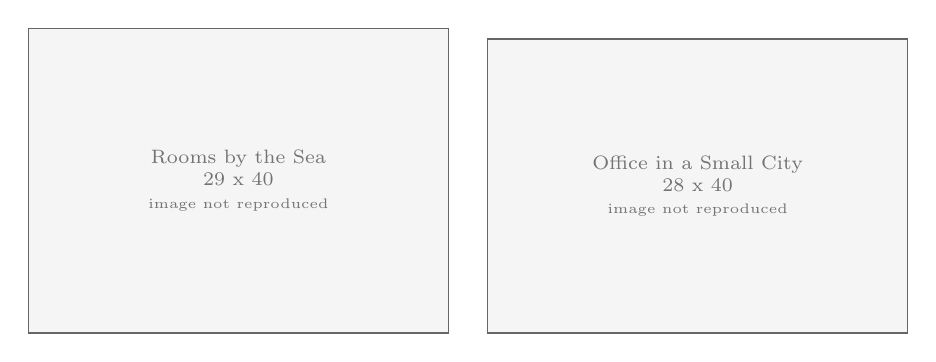
\begin{tikzpicture}
\draw[fill=black!4,draw=black!60,line width=0.5pt] (0,0) rectangle (5.333333333333333,3.8666666666666667);
\node[align=center,text=black!55,font=\scriptsize] at (2.6666666666666665,1.9333333333333333) {Rooms by the Sea\\29 x 40\\\tiny image not reproduced};
\draw[fill=black!4,draw=black!60,line width=0.5pt] (5.833333333333333,0) rectangle (11.166666666666666,3.7333333333333334);
\node[align=center,text=black!55,font=\scriptsize] at (8.5,1.8666666666666667) {Office in a Small City\\28 x 40\\\tiny image not reproduced};
\end{tikzpicture}
\caption{\textbf{Rooms by the Sea}, oil, September 1951; alias « The Jumping Off Place », 29 x 40 as the leaf writes it (Book III, leaf 41, ref 18347). Yale University Art Gallery, 1961.18.29: \url{https://lux.collections.yale.edu/view/object/63bdda22-a6be-413d-9a35-5e2649c14c21}. \textbf{Office in a Small City}, oil, September 1953, 28 x 40 as the leaf writes it (Book III, leaf 49, ref 18028). The Metropolitan Museum of Art, 53.183: \url{https://www.metmuseum.org/art/collection/search/488730}. Scale: sixty inches to eight centimetres; the two 28-by-40 and 29-by-40 formats of the studio pictures of 1949 to 1954. The frames are drawn to the proportions of the size in Edward Hopper's hand; the images are not reproduced here and can be seen at the museums' own pages. Drawn by Claude Fable~5.1, 13 September 2026, from the transcriptions and \texttt{works.json} (2026-09-13).}\label{fig:roomsoffice}
\end{figure}
